\documentclass{article}

\usepackage{arxiv}
\usepackage{amsmath, amsfonts, amssymb}
\usepackage{graphicx}
\usepackage{hyperref}
\hypersetup{hypertexnames=false,hidelinks}
\usepackage{booktabs}
\usepackage{enumitem}
\usepackage{float}
\usepackage{tikz}
\usetikzlibrary{arrows.meta, positioning, shapes.geometric, calc, fit}
\setlength{\headheight}{23pt}
\makeatletter
\def\headeright{}
\def\undertitle{}
\makeatother
\AtBeginDocument{
  \setlength{\headheight}{23pt}
  \addtolength{\topmargin}{-9pt}
}

\title{The Stewardship Pattern:\\
Maintaining Executable Intelligence Across Agent Loops}

\author{
  Josh Rosen \\
  ThruWire, Inc.
  \And
  Seth Rosen \\
  ThruWire, Inc.
}

\begin{document}

\maketitle

\begin{abstract}
Multi-agent AI systems increasingly consist of agents with their own task loops: they plan, call tools, delegate work, and produce outputs through interaction with external systems. Interoperability helps those agents communicate, but communication alone does not maintain the shared structure future agents inherit. In long-lived, dependency-bearing work, locally successful loops can accumulate cross-agent drift: stale assumptions, inconsistent artifacts, duplicated procedures, incompatible context selection, and final outputs that no longer agree with maintained upstream state.

We hypothesize that such systems can benefit from adopting the stewardship pattern: agent harnesses couple their task loops to a shared inner stewardship harness that maintains executable intelligence they can consume and collectively steward. The inner stewardship harness is an MCP-accessible executable environment for durable, versioned procedures and artifacts that future agents can run against: current artifacts, executable context patterns, supersession, authority, dependency-aware invalidation, affectedness, and stewardship integration. Agent harnesses use this structure when it applies, ask the inner harness to execute relevant structure with task inputs, consume the resulting artifacts, and propose updates when their work reveals gaps.

The contribution is a systems abstraction and reference architecture, not an empirical benchmark. We define the stewardship pattern, the inner stewardship harness, and executable context patterns; distinguish agent interoperability from maintained executable state; outline an MCP-accessible inner-harness interface; and propose evaluation criteria for testing cross-agent drift and maintained-state quality.
\end{abstract}

\section{Introduction}

Agent loops are the familiar operating pattern of contemporary agents: they explore, call tools, recover from partial failure, and adapt to a task \cite{yao2023react,schick2023toolformer,wu2023autogen,li2023camel,hong2023metagpt,wang2023voyager}. These loops run in \emph{agent harnesses}: task-facing harnesses that manage prompting, tool calls, delegation, retries, local task state, and interaction with external systems. This paper distinguishes such agent harnesses from a shared \emph{inner stewardship harness}: the executable environment that stores, runs, and maintains shared structure across many agent loops. We use \emph{outer loop} as this paper's label for the task-directed agent loop when it surrounds calls into the inner stewardship harness. The term distinguishes the agent's open-ended task loop from the inner graph nodes, materialization steps, validation checks, and recomputation paths executed by the inner harness. The same flexibility becomes a systems problem when many loops work over long-lived shared state. A locally successful loop may answer a task while leaving the maintained criteria artifact stale, invent a better procedure but preserve it only in a transcript, or retrieve a different context bundle than a peer loop. Across many agents, local task success can compound global drift.

We call this \emph{cross-agent drift}: loss of coherence as agents assemble different context, preserve different assumptions, update different artifacts, and leave authority unresolved. Agent communication is not maintained executable shared state. Agents may exchange messages fluently while still disagreeing about which artifacts are current, which procedures should run, which outputs are stale, and which changes affect downstream work.

This paper proposes the stewardship pattern for long-lived, dependency-bearing multi-agent systems: agent harnesses use an MCP-accessible inner stewardship harness that stores, runs, and maintains executable context patterns, intermediate artifacts, supersession, current-state resolution, and affectedness. \emph{Executable intelligence} is the part of shared state that future agents can run against: context patterns, artifact contracts, authority structure, dependency structure, validation steps, and materialization behavior learned over time. Outer loops are both consumers and maintainers of this structure. A stewardship-compliant loop does not first produce an independent final answer and then ask how to clean up. It asks at task selection time what structure already exists, uses the inner harness to materialize and execute relevant context patterns or graph regions, consumes the intermediate artifacts produced by that execution, and routes new observations back into maintained structure as they arise.

We present this as a design pattern in the software-architecture sense: a named, reusable solution structure for a recurring problem, documented with its context, forces, consequences, and reference implementation. This framing is intentional. The paper offers an abstraction, reference architecture, and evaluation agenda for a pattern motivated by proprietary implementation experience; it does not report a controlled benchmark of the pattern's effects.

This framing builds on prior ThruWire work on execution lineage and first-class intermediate artifacts \cite{rosen2026lineage,rosen2026artifacts}. The present paper asks how many outer loops can maintain the executable structure future loops inherit. A2A-style interoperability helps agents find and delegate to other agents \cite{a2a2026spec}; MCP provides a schema-described tool and context interface to the inner harness \cite{mcp2025intro,mcp2025tools,mcp2025resources,mcp2025prompts}. LLM-maintained wikis and Git repositories are also valuable shared-state mechanisms, but the question here is what provides executable context patterns, authority, supersession, affectedness, and stewardship validation.

The paper makes four contributions:
\begin{itemize}[leftmargin=*]
\item We define the stewardship pattern as the protocol expectation that existing agent harnesses consume current shared structure when it applies, select and run the relevant inner-harness block or graph region with task inputs, and keep the shared execution environment aligned with what the task discovers, or justify why no update was needed.
\item We define the inner stewardship harness as the shared executable environment for maintained intelligence across many outer loops.
\item We introduce executable context patterns as versioned procedures for assembling, omitting, generating, and validating the right artifacts and constraints for a class of task.
\item We provide a reference architecture, MCP-accessible inner-harness interface, lifecycle model, limitations, and evaluation agenda for measuring cross-agent drift and stewardship quality.
\end{itemize}

\begin{table}[H]
\centering
\small
\begin{tabular}{p{0.22\linewidth}p{0.68\linewidth}}
\toprule
\textbf{Pattern field} & \textbf{Stewardship pattern summary} \\
\midrule
Intent & Keep shared executable structure current and improving across many agent loops. \\
Problem & Cross-agent drift: locally successful loops can leave shared context, artifacts, procedures, authority, and downstream state inconsistent. \\
Forces & Local task success versus global coherence; flexible agent loops versus disciplined maintained state; stewardship value versus latency, review burden, and proposal noise. \\
Solution & Couple agent harnesses to one inner stewardship harness through MCP; select and execute maintained structure during work; route observations, artifact changes, affectedness, and review through the lifecycle in Section~\ref{sec:lifecycle}. \\
Participants & Outer loops, agent harnesses, inner stewardship harness, executable context patterns, maintained artifacts, and human reviewers or policy gates. \\
Consequences & Improved maintained-state discipline is possible, but the pattern introduces coordination overhead, governance requirements, false invalidation risk, pattern drift, and stewardship noise. \\
Known uses & Proprietary ThruWire systems motivate the abstraction; they are not open-sourced or used here as controlled empirical evidence. \\
\bottomrule
\end{tabular}
\caption{The stewardship pattern in compact design-pattern form.}
\label{tab:pattern-summary}
\end{table}

The authors have built proprietary systems that motivate this abstraction. This paper does not open-source those systems, describe them in sufficient detail for reproduction, or rely on them as controlled empirical evidence. The public contribution is the abstraction, terminology, reference architecture, design requirements, and evaluation agenda.

The claims are deliberately bounded. We do not claim that the stewardship pattern replaces A2A, replaces communication, eliminates drift, guarantees better final answers, or is appropriate for every task. We propose an architecture and evaluation agenda for long-lived AI work where future agents depend on maintained structure.

\section{Motivating Example: Company Intelligence and Strategy Analysis}

Consider company intelligence executed over months by multiple humans and agents: founder research, funding updates, technical novelty assessments, competitive-risk memos, criteria edits, and customer-implication reports. Each task may appear successful while the shared state degrades. One loop treats a stale market map as current; another uses a superseded rubric; another updates a final memo but leaves the technical novelty artifact unchanged.

The failure is not absence of text or memory. It is absence of maintained executable structure: a durable procedure for deciding what context to materialize, which artifacts are authoritative, which versions are superseded, which downstream artifacts depend on a criteria artifact, and what must be reviewed after change. The procedure can also encode how the task should think, not only what it should load. For company intelligence, the inner harness can require a fan-out of sealed perspective artifacts: technical read, founder and incentive read, company-stage read, market-category read, product-pattern read, narrative read, competitive-threat read, and an explicit noise or overfit check. It can require at least one artifact to argue the contrary position: why the target may not matter, why vocabulary overlap is not substance, what not to overreact to, and what evidence would change the decision.

With the stewardship pattern, the risk-assessment loop asks the inner harness for an executable context pattern:
\begin{quote}
For a competitor-risk assessment, bind the target company, reference company, peer set, market category, and stage band; load the current company model, founder and stage artifact, funding artifact, technical novelty artifact, competitive landscape, strategic priorities, open questions, and current risk criteria; omit stale market-map versions and superseded rubrics; materialize independent technical, market, product, narrative, threat, and noise-check artifacts; require the final judgment to weigh strongest evidence against strongest counterargument.
\end{quote}

The inner harness materializes current artifacts and runtime slots, then executes the reusable perspective structure as part of producing the final brief. If the loop discovers that technical novelty needs different criteria for research-heavy and services-heavy companies, stewardship means routing that observation into a context-pattern or criteria change for inner-harness execution, not merely mentioning the distinction in the final memo. If the contrary read shows that the target was mostly noise, the loop should still leave useful maintained state through the inner harness: a no-action rationale, future revisit conditions, or a deduplication note that helps future agents avoid rediscovering the same non-signal. Figure~\ref{fig:harness-architecture} sketches the architecture.

\begin{figure}[t]
\centering
\begin{tikzpicture}[
  font=\scriptsize,
  scale=0.82,
  transform shape,
  node distance=8mm,
  loop/.style={draw, rounded corners, align=center, text width=24mm, minimum height=8mm, fill=black!3},
  mcp/.style={draw, rounded corners, align=center, text width=24mm, minimum height=10mm, fill=black!6},
  harness/.style={draw, rounded corners, align=center, text width=38mm, minimum height=13mm, fill=black!4},
  store/.style={draw, rounded corners, align=center, text width=26mm, minimum height=9mm, fill=black!2},
  action/.style={draw, rounded corners, align=center, text width=25mm, minimum height=8mm, fill=black!5},
  arr/.style={-{Stealth[length=2mm]}, thick},
  dasharr/.style={-{Stealth[length=2mm]}, dashed, thick}
]
\node[loop] (loop) at (0,1.05) {outer\\agent loop};
\node[mcp] (mcp) at (3.2,1.05) {MCP\\interface};
\node[harness] (h) at (7.8,1.05) {inner stewardship harness\\executable environment};
\node[store] (g) at (12.6,2.55) {executable\\graph};
\node[store] (a) at (12.6,1.50) {artifact\\store};
\node[store] (p) at (12.6,0.45) {context-pattern\\registry};
\node[store] (pol) at (12.6,-0.60) {review and\\validation};
\node[action] (out) at (7.8,-0.75) {consume\\artifacts};
\node[action] (obs) at (0,-2.35) {observe during\\work};
\node[action] (prop) at (3.6,-2.35) {route\\update};
\node[action] (val) at (7.2,-2.35) {integrate\\state};
\node[action] (future) at (10.8,-2.35) {future loop\\inherits};

\draw[arr] (loop.east) -- (mcp.west);
\draw[arr] (mcp.east) -- (h.west);
\draw[arr] (h.east) -- (g.west);
\draw[arr] (h.east) -- (a.west);
\draw[arr] (h.east) -- (p.west);
\draw[arr] (h.east) -- (pol.west);
\draw[arr] (h.south) -- (out.north);
\draw[dasharr] (loop.south) -- (obs.north);
\draw[dasharr] (obs.east) -- (prop.west);
\draw[dasharr] (prop.east) -- (val.west);
\draw[dasharr] (val.east) -- (future.west);
\draw[dasharr] (val.north east) -- (pol.south west);
\end{tikzpicture}
\caption{Outer loops use shared executable structure through MCP while the task is being performed. The inner harness materializes context, executes graph regions, produces or registers artifacts, and integrates observations or proposed changes so future loops inherit improved maintained state.}
\label{fig:harness-architecture}
\end{figure}

\subsection{Concrete Lifecycle Trace}

A compact task trace makes the architecture operational:
\begin{enumerate}[leftmargin=*]
\item \textbf{Input task.} An outer loop receives: ``Reassess competitive risk for Company X in the infrastructure-software market.''
\item \textbf{Selection.} Through MCP, the loop searches or selects the current compiled structure for \texttt{competitor\_risk\_assessment}: a context pattern, graph region, output contract, and relevant artifact roles.
\item \textbf{Materialization.} The inner harness resolves current company, funding, technical-novelty, competitive-landscape, and risk-criteria artifacts; excludes stale maps and superseded rubrics; binds \texttt{peer\_set}, \texttt{market\_category}, and \texttt{stage\_band}; and returns a context bundle plus output contract.
\item \textbf{Perspective execution.} The inner harness executes or materializes independent lens artifacts: technical fit, product implications, strategic implications, competitive threat, narrative implications, and a contrary noise or overfit check.
\item \textbf{Task execution.} The loop consumes those artifacts, performs the open-ended judgment, and asks the inner harness to produce or register an updated risk-assessment artifact that states both the strongest evidence and strongest counterargument.
\item \textbf{Stewardship update.} If the task reveals a reusable criteria distinction, missing lens, or better contrary check, the loop records the observation and proposes a criteria or context-pattern change.
\item \textbf{Affectedness and integration.} The inner harness applies or routes the proposed change through review or publication steps, marks affected downstream artifacts stale, and validates that the task execution consumed current artifacts, produced the expected output through the artifact contract, and routed the pattern change for review if required.
\end{enumerate}

\section{Background and Related Work}

\subsection{Interoperability and Tool/Context Access}

A2A defines an interoperability layer for independent agents: discovery, task delegation, messages, artifacts, streaming, and protocol bindings \cite{a2a2026spec}. MCP connects AI applications to external systems through schema-described tools, resources, resource templates, and prompts \cite{mcp2025intro,mcp2025tools,mcp2025resources,mcp2025prompts}. In this paper, A2A routes work among agents, MCP exposes the inner harness to agent harnesses, and the stewardship pattern supplies execution-control semantics.

\subsection{Harnesses and Procedural Memory}

Agent harness work treats the harness around a model as an object of study. Natural-Language Agent Harnesses externalize control logic as editable executable artifacts with contracts, durable artifacts, and adapters \cite{pan2026nlah}; related surveys and systems emphasize planning, tool use, memory, verification, state, and control \cite{ning2026codeharness,lou2026autoharness,zhang2025harness}. Procedural-memory and workflow-memory systems preserve reusable guidance: procedures, trajectories, decompositions, and experiences that help later agents plan or act more effectively \cite{wang2024awm,fang2025memp,fan2024workflowllm,han2025legomem,yan2025memoryr1,borro2026memori}. The inner stewardship harness is different because it is stateful over the work products themselves. It maintains intermediate and final artifacts, graph or block execution state, run records, lineage, and context patterns as shared executable state. Procedural memory can suggest how a future loop should proceed; the inner harness determines what maintained artifacts and executable structures that loop should run against, update, or leave unchanged.

\subsection{Shared Knowledge and Repository Mechanisms}

LLM-maintained wikis compound synthesized knowledge over time \cite{karpathy2026llmwiki,wen2026knowledgecompounding}. Git repositories coordinate versioned files, review, rollback, attribution, and CI hooks \cite{chacon2014progit}. Knowledge graphs, vector stores, and wikis preserve shared facts, relations, notes, or retrieved memories \cite{hogan2021knowledgegraphs}. These mechanisms may store or review inner-harness inputs, but storage is not execution semantics. If \texttt{risk\_rubric.md} changes from \texttt{risk\_criteria:v1} to \texttt{risk\_criteria:v2}, Git can represent the patch and CI can run tests; the inner harness determines whether the new rubric is current for a role and scope, which context patterns use it, and which downstream artifacts consumed the old rubric.

\begin{table}[H]
\centering
\scriptsize
\begin{tabular}{p{0.16\linewidth}p{0.21\linewidth}p{0.26\linewidth}p{0.21\linewidth}}
\toprule
\textbf{Mechanism} & \textbf{Primary durable object} & \textbf{Good at} & \textbf{Not primary unless extended} \\
\midrule
LLM-maintained wiki & Markdown pages, summaries, links, indexes & Shared accumulated knowledge and synthesis & Runtime slots, artifact authority, invalidation, recomputation as first-class protocol semantics \\
Git repository & Versioned files, commits, branches, diffs, pull requests & Shared review, history, rollback, CI integration & Semantic current-state resolution for LLM-native artifacts as the agent-facing protocol \\
Vector memory & Embeddings and retrieved memories & Recall and similarity-based reuse & Explicit dependency structure and supersession as primary abstractions \\
Knowledge graph & Entities and relations & Structured factual and relational knowledge & Executable context procedures and affectedness as primary abstractions \\
Inner stewardship harness & Context patterns, artifacts, graph state, review structure, runtime records & Maintained executable intelligence across loops & Requires schema, governance, and stewardship discipline \\
\bottomrule
\end{tabular}
\caption{Adjacent shared-state mechanisms can support the stewardship pattern, but do not by themselves define the agent-facing stewardship protocol proposed here unless extended with additional semantics.}
\label{tab:shared-state-mechanisms}
\end{table}

\subsection{Blackboards, Workflow DAGs, Provenance, and Multi-Agent Frameworks}

Blackboard systems identify the value of a shared workspace where multiple specialists contribute partial results \cite{nii1986blackboard}. They are a useful historical analogy for agent systems because they separate local specialist behavior from shared intermediate state. The inner stewardship harness differs by making the shared state executable, versioned, and dependency-bearing rather than only a posted working memory.

Workflow systems such as Dryad, Spark, Airflow, and dbt use dependency structure, materialized intermediates, and lineage-aware execution \cite{isard2007dryad,zaharia2010spark,airflowdocs,dbtdocs}; provenance research studies why and where outputs arise from prior state \cite{buneman2001why,freire2008provenance}. These systems are closest to the paper's execution-lineage foundation, but they usually coordinate data or software workflows rather than agent loops that discover and revise context patterns while performing open-ended work.

Multi-agent frameworks such as CAMEL, AutoGen, MetaGPT, Voyager, and Magentic-One organize agents into roles, conversations, planners, and tool users \cite{li2023camel,wu2023autogen,hong2023metagpt,wang2023voyager,fourney2024magenticone}. They help structure agent teams and task execution. The stewardship pattern addresses a different layer: the maintained executable state those agents consume, update, and validate across many runs.

\section{Problem Formulation}

\subsection{Outer Loops}

An \emph{outer loop} is the paper's term for the agentic task loop, running inside an agent harness, that surrounds calls into the inner stewardship harness. In common agent terminology, this is simply an agent loop: it plans, calls tools, reasons, delegates, observes, and completes a task. We treat it as the accountable unit because it consumes task context, acts, and decides what observations, inputs, or proposed structural changes should be returned to the shared execution environment.

Let $C=\{c_1,\ldots,c_n\}$ be clients, agent harnesses, or outer loops. Each loop $c_i$ receives a task objective $\tau_i$ and a materialized context bundle $b_i$. It performs open-ended work and may produce messages, tool calls, draft judgments, observations, or proposed mutations. Maintained artifacts are created or registered by the inner harness according to artifact contracts and compiled review or publication structure. Without the stewardship pattern, the loop's natural optimization target is isolated task completion:
\begin{equation}
c_i: (\tau_i, b_i) \rightarrow y_i
\end{equation}
where $y_i$ is an isolated task output. Isolated completion does not imply maintained shared state.

\subsection{Architectural Objective}

The architectural objective is to reduce drift accumulation across repeated tasks while preserving task-completion performance. In long-lived workloads with dependency-bearing artifacts, the hypothesis is that executable stewardship improves maintained-state quality: fewer stale current artifacts, fewer duplicated procedures, more consistent context materialization, and more accurate affectedness after changes. This is structural, not a claim that the stewardship pattern makes models smarter. Future evaluations should measure both drift reduction and the added latency, review burden, and proposal noise.

\subsection{Cross-Agent Drift}

Cross-agent drift occurs when many locally successful loops cause shared state to become less coherent. We distinguish five forms:
\begin{itemize}[leftmargin=*]
\item \textbf{Context drift:} different loops assemble incompatible context bundles for similar tasks.
\item \textbf{Artifact drift:} final outputs are updated while upstream intermediate artifacts remain stale.
\item \textbf{Procedure drift:} loops evolve incompatible task procedures or criteria.
\item \textbf{Authority drift:} multiple artifacts are treated as current without explicit resolution.
\item \textbf{Evaluation drift:} loops optimize isolated task outputs without maintaining reusable structure.
\end{itemize}

These failures can occur even when every loop appears competent. The missing element is a maintained execution environment that makes shared state legible, current, and improvable.

\subsection{Observed Failure Patterns}

The failure modes above are not experimental results in this paper. They are illustrative patterns that motivate the proposed architecture and that future evaluations should measure directly.

\begin{table}[H]
\centering
\small
\begin{tabular}{p{0.24\linewidth}p{0.64\linewidth}}
\toprule
\textbf{Failure pattern} & \textbf{Typical behavior in loop-centric systems} \\
\midrule
Artifact drift & A final report is updated, but the criteria artifact or intermediate analysis it depends on remains stale. \\
Procedure drift & Two agents independently evolve different evaluation rubrics for similar tasks and preserve them only in isolated outputs or transcripts. \\
Authority drift & Multiple summaries, rubrics, or analyses are treated as current because no role/scope-specific resolver selects the active artifact. \\
Context drift & Similar tasks materialize different context bundles because each loop performs ad hoc retrieval or uses a different memory fragment. \\
Evaluation drift & Agents optimize the visible final answer but do not update reusable procedures, validation steps, or dependency structure. \\
Stewardship noise & Many agents propose low-value observations, criteria edits, or pattern changes, increasing review burden without improving maintained state. \\
\bottomrule
\end{tabular}
\caption{Illustrative failure patterns that the stewardship pattern is intended to make visible and measurable.}
\label{tab:failure-patterns}
\end{table}

\subsection{Why Shared Memory and A2A Are Insufficient Alone}

Shared memory can improve recall, and A2A can route work to a capable agent, but neither by itself defines artifact authority, supersession, context materialization, or downstream affectedness. In long-lived settings, loops need a layer where they can inspect and improve shared executable state.

\section{Inner Stewardship Harness}

\subsection{Definition}

We define an inner stewardship harness as:
\begin{equation}
\mathcal{H} = (G, A, P, R, C, \Pi)
\end{equation}
where:
\begin{itemize}[leftmargin=*]
\item $G$ is executable graph structure: blocks, steps, tasks, and dependency edges.
\item $A$ is maintained artifact state: intermediate and final artifacts, versions, statuses, lineage, authority scope, and supersession records.
\item $P$ is the set of executable context patterns.
\item $R$ is the set of runtime records: executions, inputs, slots, resolved dependencies, validations, and materialization events.
\item $C$ is the set of clients, agent harnesses, or outer loops accessing the inner harness through MCP.
\item $\Pi$ is policy: permissions, approval, supersession, invalidation, validation, conflict handling, and review requirements.
\end{itemize}

The inner stewardship harness is inner because many agent harnesses call into it while performing task-facing work. It is a stewardship harness because it maintains the executable knowledge layer future loops inherit. In consumer mode, a loop resolves the relevant pattern, artifacts, graph nodes, compiled version, and slots, then asks the inner harness to run the selected block or graph region with task inputs. In steward mode, the loop returns observations, evidence, and proposed changes to criteria, dependencies, context patterns, or validation steps; the inner harness applies, routes, or rejects those changes through its compiled review and publication structure.

\subsection{Execution Control Plane}

The \emph{execution control plane} determines what is current, stale, reusable, recomputable, reviewable, or accepted into maintained state. It answers questions such as:
\begin{itemize}[leftmargin=*]
\item Which artifact is current for this role and scope?
\item Which downstream artifacts become stale after this supersession?
\item Which context pattern should be used for this goal type?
\item Which existing graph region or artifact contract should this task execute against?
\item Which proposed graph mutation violates a dependency or authority boundary?
\item Which affected subgraph should be recomputed, reviewed, or left unchanged?
\end{itemize}

\subsection{Artifacts, Current State, and Supersession}

Following artifact-centric state, artifacts in $A$ are typed, addressable, versioned, dependency-aware, and consumable by downstream computation \cite{rosen2026artifacts}. Each artifact has a role, scope, lineage, status, and authority boundary. A superseding artifact can replace an earlier artifact as current for a role and scope while preserving audit history.

Current-state resolution is therefore a maintained operation:
\begin{equation}
\mathrm{current}(role, scope, t) \rightarrow a_k
\end{equation}
where $a_k$ is the artifact that the execution control plane considers active at time $t$ according to $\Pi$. If no artifact is current, or if multiple candidates conflict, the inner harness should surface that condition rather than letting each outer loop infer authority locally.

The hard case is authority resolution. Because maintained artifacts are produced or registered by inner-harness execution, conflicts should not be modeled as arbitrary outer loops writing competing current artifacts. They arise when two inner-harness runs, graph versions, criteria revisions, or review decisions could each make a different artifact current, or when an artifact is current for one scope but not another. Implementations may use human review, trust tiers, confidence thresholds, ownership metadata, or deterministic resolution steps such as preferring approved runs over draft runs. If the compiled review or publication structure cannot resolve the conflict, artifact reads and current-state queries should surface a structured unresolved or missing state rather than a silent guess.

\subsection{Invalidation and Propagation}

If artifact $a$ is superseded by $a'$, every downstream artifact whose execution identity depended on $a$ may require invalidation, recomputation, or review. The inner harness should support:
\begin{itemize}[leftmargin=*]
\item exact preservation of unaffected branches,
\item stale marking before recomputation,
\item selective recomputation of affected descendants,
\item review nodes for high-authority or high-risk updates,
\item publication of superseding artifacts when recomputation completes.
\end{itemize}

This preserves the execution-lineage distinction between final output quality and maintained-state quality.

\section{Minimum Viable Inner Stewardship Harness}

The smallest useful inner harness should include:
\begin{itemize}[leftmargin=*]
\item an artifact registry with role, scope, version, status, lineage, and authority metadata,
\item a current-state resolver for \texttt{current(role, scope, t)},
\item a context-pattern registry with versioned selection, exclusion, slot, and output-contract declarations,
\item a materialization function that binds inputs and slots and returns a context bundle with provenance,
\item supersession and stale-marking operations,
\item validation or integration steps for task completion,
\item optional human review nodes for high-authority changes.
\end{itemize}

This minimum version excludes general agent-to-agent communication, broad social negotiation, full workflow orchestration, automatic proof that all dependencies were found, and automatic acceptance of agent-proposed pattern changes. Even a small inner harness should make current state explicit, make context materialization executable, record supersession, and support stewardship integration throughout task execution.

\section{Executable Context Patterns}

\subsection{Definition}

A \emph{context pattern} is an executable, versioned procedure for assembling the right context for a class of task. It is not just a prompt template and not just retrieval. A context pattern declares which artifacts, sources, roles, constraints, inputs, and slots should be loaded, omitted, generated, refreshed, or validated at runtime.

We define a context pattern as:
\begin{equation}
p = (g, I, S, Q, M, E, V, O)
\end{equation}
where:
\begin{itemize}[leftmargin=*]
\item $g$ is the goal type, such as competitor-risk assessment.
\item $I$ is the input schema.
\item $S$ is the slot schema for runtime bindings.
\item $Q$ is the set of selection declarations for artifacts, sources, and roles.
\item $M$ is the set of generation or materialization steps.
\item $E$ is the set of exclusion declarations.
\item $V$ is the set of validation steps or review nodes.
\item $O$ is the output contract.
\end{itemize}

A pattern is executable because it accepts runtime inputs and slots, resolves current artifacts, may materialize generated intermediates, and returns a bounded context bundle with provenance.

\subsection{Example}

For a company-risk assessment, a context pattern might be:
\begin{itemize}[leftmargin=*]
\item \textbf{Goal type:} competitor-risk assessment.
\item \textbf{Inputs:} target company, assessment date, requested risk lens.
\item \textbf{Slots:} peer set, market category, prior thesis, stage band.
\item \textbf{Selection declarations:} load current company profile, founder/stage artifact, funding artifact, technical novelty artifact, comparable-company pattern artifact, and current risk criteria.
\item \textbf{Exclusion declarations:} omit stale market-map versions, superseded risk rubrics, unrelated prior summaries, and artifacts outside the target market category.
\item \textbf{Generation steps:} materialize peer-set comparison and risk-criteria checklist at runtime.
\item \textbf{Validation steps:} resolve current state for each authoritative artifact; flag missing technical novelty state.
\item \textbf{Output contract:} produce or register a risk assessment artifact with role, scope, lineage, confidence, supersession target if any, and downstream dependents.
\end{itemize}

This pattern encodes context precision: load these artifacts but not those artifacts; generate this intermediate only after slots are bound; reject or review the task if the authoritative criteria artifact is missing. The pattern is learned structure, not merely a longer prompt.

\subsection{How Patterns Improve}

Outer loops improve context patterns when they discover that a pattern is incomplete, overloaded, stale, too broad, too narrow, or reusable in a stronger form. The company-risk example in Section~2 illustrates the expected behavior: the loop turns a procedural discovery into a criteria update, slot, branch, or validation step rather than preserving it only in the final memo.

Pattern improvement should be reviewable. Bad patterns can propagate mistakes by making future loops confidently load the wrong context. The inner harness therefore needs versioning, evidence, validation steps, rollback or supersession, and review or publication structure for pattern changes.

\section{MCP as the Inner-Harness Interface}

\subsection{Harness Surface}

MCP is a natural interface because it lets heterogeneous agent harnesses access the same inner harness without sharing one internal architecture. The important point is not that the inner harness exposes a large collection of isolated tools. The MCP surface is a control surface for a maintained system: projects, blocks, folders, compiled versions, executable graph state, runs, event streams, artifacts, and review or publication steps. Ordinary-looking operations such as reading a block, compiling a version, running a block, polling run events, and reading an artifact become stewardship operations when they participate in compiled structure that carries lineage, authority, slots, cached context, and publication behavior.

The exact tool names are implementation-specific. An inner harness may expose semantic operations directly, or realize them through lower-level project, block, version, run, and artifact operations. The useful surface groups capabilities by function:
\begin{itemize}[leftmargin=*]
\item \textbf{Discovery and selection:} list projects, folders, blocks, context patterns, graph nodes, and available artifacts; search compiled structure when the loop does not know the exact block to run.
\item \textbf{Authoring and mutation:} read, create, edit, move, rename, or delete raw blocks and folders through the inner harness's authoring surface; propose graph or context-pattern changes as structured mutations rather than transcript notes.
\item \textbf{Compilation and versioning:} compile raw structure into an immutable executable version; resolve the current compiled version; preserve prior versions for audit, rollback, and affectedness analysis.
\item \textbf{Execution and materialization:} run a selected block or graph region with runtime inputs and slot bindings; materialize the context bundle, intermediate artifacts, final artifacts, and provenance implied by that run.
\item \textbf{Observation and integration:} stream or poll run events, inspect produced artifacts, record observations, run review or publication blocks, mark affected state stale, and execute the stewardship-integration structure for the task.
\end{itemize}

The design requirement is that a loop can discover or select an existing executable graph region, run it with task-specific inputs and slots, consume the resulting context and artifacts, and integrate observations or proposed edits into maintained structure through schema-described operations. In some implementations, high-level materialization or integration operations may be exposed directly. In others, those semantics emerge from compiling a graph, running selected blocks, resolving artifacts, inspecting run events, and executing review or publication steps encoded in the graph. Both are inner-harness designs, not merely tool collections.

\subsection{Harness Operation Sketches}

The following sketches are illustrative and use generic operations for a compiled-block inner harness: search compiled blocks, inspect the current DAG, read current artifacts, execute blocks, poll run events, edit raw blocks, and compile a new version. They should not be read as a separate rule engine or as a claim that every implementation exposes these exact names. Checks and constraints are expressed through executable blocks, compiled graph structure, artifact contracts, run events, and review or publication steps.

\begin{verbatim}
select_current_structure(goal, inputs):
  matches = search_compiled_blocks(query=goal)
  dag = get_current_dag()
  return choose_block_or_graph_region(matches, dag, inputs)

consume_current_artifact(block_id, inputs, slot_bindings):
  result = read_current_artifact(block_id, inputs, slot_bindings)
  if result.status == "success": return result.artifact
  return result  // e.g., missing artifact or slot-binding guidance

run_structured_work(block_id, inputs, slot_bindings):
  accepted = run_block(block_id, inputs, slot_bindings)
  events = poll_run_events(accepted.run_id)
  return {run_id: accepted.run_id, events: events}

inspect_outputs(block_id, inputs, slot_bindings):
  artifact = read_current_artifact(block_id, inputs, slot_bindings)
  artifacts = list_current_artifacts()
  return {artifact: artifact, project_artifacts: artifacts}

steward_structure(block_path, revised_block):
  existing = read_raw_block(block_path)
  upsert_raw_block(block_path, revised_block)
  compiled = compile_project_version()
  return {previous: existing.revision, version: compiled.version_id}
\end{verbatim}

\subsection{Relationship to A2A}

A2A routes work among agents; MCP exposes the inner harness to those agents and their agent harnesses; the inner harness maintains execution semantics through its project, graph, version, run, artifact, and review/publication machinery. Table~\ref{tab:layers} summarizes the boundary.

\begin{table}[H]
\centering
\small
\begin{tabular}{p{0.20\linewidth}p{0.34\linewidth}p{0.34\linewidth}}
\toprule
\textbf{Layer} & \textbf{Solves} & \textbf{Boundary} \\
\midrule
A2A & Agent discovery, delegation, task exchange, and message-level interoperability. & Shared maintained intelligence, artifact authority, or dependency-aware invalidation as its primary abstraction. \\
MCP & Schema-described access to inner-harness operations, resources, runs, artifacts, and context. & Maintained-state semantics unless backed by an inner harness or equivalent application layer. \\
Inner stewardship harness & Current state, durable artifacts, executable context patterns, compiled versions, runs, supersession, and propagation. & General communication, social negotiation, or all agent-to-agent coordination as its primary role. \\
\bottomrule
\end{tabular}
\caption{A2A, MCP, and the inner stewardship harness operate at complementary layers.}
\label{tab:layers}
\end{table}

The two layers can compose. An A2A client may delegate a task to a specialized agent. That agent may then use MCP to materialize context from the inner harness, execute the task with inner-harness-produced intermediates, ask the inner harness to produce or register artifacts, and integrate stewardship updates before returning an A2A artifact. A2A helps route the task to the right agent. Context patterns help the selected agent inherit the right structure.

\section{Integrated Stewardship Lifecycle}
\label{sec:lifecycle}

\begin{figure}[t]
\centering
\begin{tikzpicture}[
  font=\scriptsize,
  node distance=5mm,
  lifestep/.style={draw, rounded corners, align=center, text width=30mm, minimum height=8mm, fill=black!3},
  decision/.style={draw, diamond, aspect=2.2, align=center, text width=25mm, inner sep=1mm, fill=black!4},
  arr/.style={-{Stealth[length=2mm]}, thick}
]
\node[lifestep] (task) {task};
\node[lifestep, below=of task] (match) {select structure};
\node[lifestep, below=of match] (mat) {materialize context};
\node[lifestep, below=of mat] (work) {execute with\\inner-harness artifacts};
\node[decision, below=of work] (obs) {observation?};
\node[lifestep, below left=8mm and 11mm of obs] (justify) {record no-update\\justification};
\node[lifestep, below right=8mm and 11mm of obs] (propose) {route update};
\node[lifestep, below=18mm of obs] (affect) {affectedness\\analysis};
\node[lifestep, below=of affect] (validate) {run review or\\integration steps};
\node[lifestep, below=of validate] (accept) {accept current\\state};

\draw[arr] (task) -- (match);
\draw[arr] (match) -- (mat);
\draw[arr] (mat) -- (work);
\draw[arr] (work) -- (obs);
\draw[arr] (obs) -- node[above left] {no} (justify);
\draw[arr] (obs) -- node[above right] {yes} (propose);
\draw[arr] (justify) |- (affect);
\draw[arr] (propose) |- (affect);
\draw[arr] (affect) -- (validate);
\draw[arr] (validate) -- (accept);
\end{tikzpicture}
\caption{Stewardship is integrated into task execution. The outer loop selects and runs harness structure early, consumes generated artifacts while doing the work, and routes observations through affectedness, review, and integration steps before current state is accepted.}
\label{fig:stewardship-integration}
\end{figure}

At task selection time, the outer loop asks whether the inner harness already contains relevant executable structure: a context pattern, graph region, artifact contract, validation step, or recomputation path. If so, the loop asks the inner harness to run the selected structure with its inputs, parameters, and slots, then consumes the resulting artifacts, generated intermediates, validation warnings, and provenance. The resulting answer is therefore not purely local; it is produced by collaboration between the outer loop's open-ended reasoning and the inner harness's maintained executable structure.

During execution, the loop remains flexible: it may call tools, delegate subtasks, inspect artifacts, and explore. The inner harness remains active as the task proceeds by materializing intermediates, executing selected blocks, recording run events, resolving artifacts, and making missing context, overloaded context, stale artifacts, ambiguous authority, or reusable procedural discoveries available as candidate improvements rather than side notes.

As work proceeds, the loop and harness should integrate evidence and proposed changes into maintained state:
\begin{itemize}[leftmargin=*]
\item updated intermediate artifacts to be produced or registered through inner-harness execution,
\item final artifact supersessions to be accepted through review or publication structure,
\item graph dependency edits,
\item context-pattern improvements,
\item validation-step changes,
\item stale markings or recomputation requests,
\item explicit ``no shared update needed'' justifications.
\end{itemize}

A task that bypasses this integrated process can still be locally useful, but the produced answer may not be aligned with maintained state. The inner harness validates whether the task execution consumed current artifacts, left stale state, exposed unresolved authority conflicts, affected downstream dependents, or discovered reusable procedure improvements that should be routed into maintained structure. Future loops then inherit the revised shared execution environment.

\section{Evaluation Agenda}

This paper does not report a new experiment and should not be read as empirical validation. It proposes a systems abstraction, terminology, design requirements, and reference architecture. Future work should test whether the stewardship pattern reduces cross-agent drift and improves maintained-state quality under multi-loop workloads.

\subsection{Metrics}

The metrics should evaluate maintained execution state, not only final prose quality:
\begin{itemize}[leftmargin=*]
\item \textbf{Context-pattern quality:} reuse rate, improvement acceptance rate, context precision and recall, duplicate procedure creation, and future-agent lift from prior pattern improvements.
\item \textbf{Artifact-state quality:} stale artifact rate, authority conflicts, stale or superseded artifact consumption, invalidation correctness, propagation completeness, and cross-agent consistency.
\item \textbf{Stewardship behavior:} useful update rate, no-update-needed justifications, human review burden, proposal acceptance and rejection, stewardship-noise rate, time to identify affected subgraphs, and drift accumulation over $N$ tasks.
\item \textbf{Wiki and repository comparison:} stale page or file consumption, rediscovered procedures despite shared content, updates that become executable context-pattern changes, time to assess downstream impact, file changes without affectedness metadata, and future-loop use of the correct current artifact.
\end{itemize}

\subsection{Proposed Benchmark Design}

A small benchmark can make the hypothesis falsifiable without requiring a full product-scale deployment. One design is a repeated company-intelligence or research-synthesis workload with evolving criteria. Each trial would run a sequence of related tasks and introduce a legitimate criteria change midway through the sequence.

The comparison conditions should include:
\begin{itemize}[leftmargin=*]
\item independent agent loops with ad hoc retrieval,
\item a shared LLM-maintained wiki,
\item a shared Git repository of markdown pages, prompts, policies, and tests,
\item shared memory or vector retrieval,
\item A2A-style delegation without the stewardship pattern,
\item MCP-mediated stewardship over maintained artifacts and context patterns.
\end{itemize}

The benchmark should measure stale artifact rate, context consistency across agents, duplicate procedure creation, affectedness accuracy, review burden, and future-agent reuse. The expected result is not assumed. A shared wiki or repository may perform well on recall and reuse; the stewardship pattern should be judged specifically on maintained-state metrics such as current artifact resolution, invalidation correctness, propagation completeness, context-pattern consistency, and stewardship integration.

Other task families include strategy planning with evolving criteria, codebase maintenance where requirements and verification artifacts must remain aligned, and multi-agent competitive analysis where context patterns determine which static and generated artifacts enter context. Future experiments should avoid claiming that the stewardship pattern makes models smarter or guarantees better final answers. The appropriate hypotheses are structural:
\begin{itemize}[leftmargin=*]
\item fewer completed tasks leave stale authoritative artifacts,
\item affected subgraphs are identified more quickly and accurately,
\item future loops assemble more consistent context bundles,
\item useful procedural improvements are reused rather than rediscovered,
\item final outputs agree more often with maintained upstream state.
\end{itemize}

\section{Consequences and Limitations}

The proposed architecture has important limits.

\begin{itemize}[leftmargin=*]
\item \textbf{Latency and coordination overhead.} Context matching, current-state resolution, validation, and review can slow down work that would otherwise be completed locally.
\item \textbf{Not every task justifies the machinery.} Exploratory, one-off, low-stakes, or rapidly changing tasks may be better served by ad hoc agent work, ordinary communication, or simple shared notes.
\item \textbf{Bad structure and pattern drift.} A flawed context pattern, incorrect authority decision, or overfit procedure may make future loops consistently wrong.
\item \textbf{False invalidations and missed dependencies.} Overbroad affectedness can create unnecessary recomputation and review; omitted dependencies can leave stale artifacts active.
\item \textbf{Stewardship noise and governance bottlenecks.} Many agents may propose edits, pattern diffs, stale markings, and invalidations. Without thresholds, deduplication, batching, ownership metadata, and review queues, stewardship activity can become noise or concentrate into slow approval queues.
\item \textbf{Private model reasoning should not be persisted.} The inner harness maintains artifacts, context patterns, validations, and provenance, not hidden chain-of-thought.
\item \textbf{Communication remains necessary.} A2A, chat, review comments, and human discussion still matter; the stewardship pattern does not replace them.
\item \textbf{Evaluation remains future work.} The paper provides an agenda and architecture, not benchmark results.
\end{itemize}

\section{Conclusion}

As agent systems scale from one loop to many long-lived, dependency-bearing loops, the central problem may become not only how agents talk, delegate, or remember, but what shared executable structure they can consume and collectively maintain. LLM-maintained wikis and shared repositories show that agents can accumulate knowledge and coordinate over durable files. The stewardship pattern builds on that intuition but changes the maintained object: what future loops should execute, which artifacts are current, what has become stale, and how task execution updates the shared execution environment.

We proposed the stewardship pattern for multi-agent AI systems with long-lived shared state: agent harnesses use an MCP-accessible inner stewardship harness to consume, execute, and improve shared executable structure. A2A lets agents find and communicate with other agents; MCP lets outer loops access the inner harness; the inner harness maintains artifacts, context patterns, authority, supersession, invalidation, affectedness, and stewardship integration.

The hypothesis behind the stewardship pattern is that multi-agent systems become more capable not only by adding more agents, but by giving those agents shared executable structure that compounds across tasks. When each loop can consume maintained structure and improve it during execution, the system can accumulate usable procedure, context, and artifact state rather than merely accumulating messages or outputs. This may allow long-lived agent teams to approach problems whose complexity exceeds what any single loop can reliably reconstruct from scratch.

This remains a proposal and evaluation agenda: multi-agent systems should be evaluated not only by whether a task was completed, but by whether the next agent inherits better maintained executable state.

\begin{thebibliography}{99}

\bibitem{rosen2026lineage}
Josh Rosen and Seth Rosen.
\newblock From Agent Loops to Deterministic Graphs: Execution Lineage for Reproducible AI-Native Work.
\newblock arXiv:2605.06365, 2026.

\bibitem{rosen2026artifacts}
Josh Rosen and Seth Rosen.
\newblock Intermediate Artifacts as First-Class Citizens: A Data Model for Durable Intermediate Artifacts in Agentic Systems.
\newblock arXiv:2605.12087, 2026.

\bibitem{a2a2026spec}
Agent2Agent Project.
\newblock Agent2Agent (A2A) Protocol Specification, version 1.0.0.
\newblock \url{https://a2a-protocol.org/latest/specification}, accessed June 11, 2026.

\bibitem{mcp2025intro}
Model Context Protocol.
\newblock What is the Model Context Protocol (MCP)?
\newblock \url{https://modelcontextprotocol.io/docs/getting-started/intro}, accessed June 11, 2026.

\bibitem{mcp2025tools}
Model Context Protocol.
\newblock Specification 2025-06-18: Tools.
\newblock \url{https://modelcontextprotocol.io/specification/2025-06-18/server/tools}, accessed June 11, 2026.

\bibitem{mcp2025resources}
Model Context Protocol.
\newblock Specification 2025-06-18: Resources.
\newblock \url{https://modelcontextprotocol.io/specification/2025-06-18/server/resources}, accessed June 11, 2026.

\bibitem{mcp2025prompts}
Model Context Protocol.
\newblock Specification 2025-06-18: Prompts.
\newblock \url{https://modelcontextprotocol.io/specification/2025-06-18/server/prompts}, accessed June 11, 2026.

\bibitem{yao2023react}
Shunyu Yao, Jeffrey Zhao, Dian Yu, Nan Du, Izhak Shafran, Karthik Narasimhan, and Yuan Cao.
\newblock ReAct: Synergizing Reasoning and Acting in Language Models.
\newblock In \emph{International Conference on Learning Representations}, 2023.

\bibitem{schick2023toolformer}
Timo Schick, Jane Dwivedi-Yu, Roberto Dess\`i, Roberta Raileanu, Maria Lomeli, Eric Hambro, Luke Zettlemoyer, Nicola Cancedda, and Thomas Scialom.
\newblock Toolformer: Language Models Can Teach Themselves to Use Tools.
\newblock In \emph{Advances in Neural Information Processing Systems}, 2023.

\bibitem{li2023camel}
Guohao Li, Hasan Abed Al Kader Hammoud, Hani Itani, Dmitrii Khizbullin, and Bernard Ghanem.
\newblock CAMEL: Communicative Agents for ``Mind'' Exploration of Large Language Model Society.
\newblock arXiv:2303.17760, 2023.

\bibitem{wu2023autogen}
Qingyun Wu, Gagan Bansal, Jieyu Zhang, Yiran Wu, Beibin Li, Erkang Zhu, Li Jiang, Xiaoyun Zhang, Shaokun Zhang, Jiale Liu, Ahmed Hassan Awadallah, Ryen W. White, Doug Burger, and Chi Wang.
\newblock AutoGen: Enabling Next-Gen LLM Applications via Multi-Agent Conversation.
\newblock arXiv:2308.08155, 2023.

\bibitem{hong2023metagpt}
Sirui Hong, Mingchen Zhuge, Jiaqi Chen, Xiawu Zheng, Yuheng Cheng, Ceyao Zhang, Jinlin Wang, Zili Wang, Steven Ka Shing Yau, Zijuan Lin, Liyang Zhou, Chenyu Ran, Lingfeng Xiao, Chenglin Wu, and J\"urgen Schmidhuber.
\newblock MetaGPT: Meta Programming for a Multi-Agent Collaborative Framework.
\newblock arXiv:2308.00352, 2023.

\bibitem{wang2023voyager}
Guanzhi Wang, Yuqi Xie, Yunfan Jiang, Ajay Mandlekar, Chaowei Xiao, Yuke Zhu, Linxi Fan, and Anima Anandkumar.
\newblock Voyager: An Open-Ended Embodied Agent with Large Language Models.
\newblock arXiv:2305.16291, 2023.

\bibitem{fourney2024magenticone}
Adam Fourney, Gagan Bansal, Hussein Mozannar, Cheng Tan, Eduardo Salinas, Erkang Zhu, Friederike Niedtner, Grace Proebsting, Griffin Bassman, Jack Gerrits, Jacob Alber, Peter Chang, Ricky Loynd, Robert West, Victor Dibia, Ahmed Awadallah, Ece Kamar, Rafah Hosn, and Saleema Amershi.
\newblock Magentic-One: A Generalist Multi-Agent System for Solving Complex Tasks.
\newblock arXiv:2411.04468, 2024.

\bibitem{pan2026nlah}
Linyue Pan, Lexiao Zou, Shuo Guo, Jingchen Ni, and Hai-Tao Zheng.
\newblock Natural-Language Agent Harnesses.
\newblock arXiv:2603.25723, 2026.

\bibitem{ning2026codeharness}
Xuying Ning, Katherine Tieu, Dongqi Fu, Tianxin Wei, Zihao Li, Yuanchen Bei, Jiaru Zou, Mengting Ai, Zhining Liu, Ting-Wei Li, Lingjie Chen, Yanjun Zhao, Ke Yang, Bingxuan Li, Cheng Qian, Gaotang Li, Xiao Lin, Zhichen Zeng, Ruizhong Qiu, Sirui Chen, Yifan Sun, Xiyuan Yang, Ruida Wang, Rui Pan, Chenyuan Yang, Dylan Zhang, Liri Fang, Zikun Cui, Yang Cao, Pan Chen, Dorothy Sun, Ren Chen, Mahesh Srinivasan, Nipun Mathur, Yinglong Xia, Hong Li, Hong Yan, Pan Lu, Lingming Zhang, Tong Zhang, Hanghang Tong, and Jingrui He.
\newblock Code as Agent Harness.
\newblock arXiv:2605.18747, 2026.

\bibitem{lou2026autoharness}
Xinghua Lou, Miguel L\'azaro-Gredilla, Antoine Dedieu, Carter Wendelken, Wolfgang Lehrach, and Kevin P. Murphy.
\newblock AutoHarness: Improving LLM Agents by Automatically Synthesizing a Code Harness.
\newblock arXiv:2603.03329, 2026.

\bibitem{zhang2025harness}
Yuxuan Zhang, Haoyang Yu, Lanxiang Hu, Haojian Jin, and Hao Zhang.
\newblock General Modular Harness for LLM Agents in Multi-Turn Gaming Environments.
\newblock arXiv:2507.11633, 2025.

\bibitem{wang2024awm}
Zora Zhiruo Wang, Jiayuan Mao, Daniel Fried, and Graham Neubig.
\newblock Agent Workflow Memory.
\newblock arXiv:2409.07429, 2024.

\bibitem{fang2025memp}
Runnan Fang, Yuan Liang, Xiaobin Wang, Jialong Wu, Shuofei Qiao, Pengjun Xie, Fei Huang, Huajun Chen, and Ningyu Zhang.
\newblock Memp: Exploring Agent Procedural Memory.
\newblock arXiv:2508.06433, 2025.

\bibitem{fan2024workflowllm}
Shengda Fan, Xin Cong, Yuepeng Fu, Zhong Zhang, Shuyan Zhang, Yuanwei Liu, Yesai Wu, Yankai Lin, Zhiyuan Liu, and Maosong Sun.
\newblock WorkflowLLM: Enhancing Workflow Orchestration Capability of Large Language Models.
\newblock arXiv:2411.05451, 2024.

\bibitem{han2025legomem}
Dongge Han, Camille Couturier, Daniel Madrigal Diaz, Xuchao Zhang, Victor R\"uhle, and Saravan Rajmohan.
\newblock LEGOMem: Modular Procedural Memory for Multi-Agent LLM Systems for Workflow Automation.
\newblock arXiv:2510.04851, 2025.

\bibitem{yan2025memoryr1}
Sikuan Yan, Xiufeng Yang, Zuchao Huang, Ercong Nie, Zifeng Ding, Zonggen Li, Xiaowen Ma, Hinrich Sch\"utze, Volker Tresp, and Yunpu Ma.
\newblock Memory-R1: Enhancing Large Language Model Agents to Manage and Utilize Memories via Reinforcement Learning.
\newblock arXiv:2508.19828, 2025.

\bibitem{borro2026memori}
Luiz C. Borro, Luiz A. B. Macarini, Gordon Tindall, Michael Montero, and Adam B. Struck.
\newblock Memori: A Persistent Memory Layer for Efficient, Context-Aware LLM Agents.
\newblock arXiv:2603.19935, 2026.

\bibitem{karpathy2026llmwiki}
Andrej Karpathy.
\newblock LLM Wiki.
\newblock GitHub Gist, 2026.
\newblock \url{https://gist.github.com/karpathy/442a6bf555914893e9891c11519de94f}, accessed June 11, 2026.

\bibitem{wen2026knowledgecompounding}
Shuide Wen and Beier Ku.
\newblock Knowledge Compounding: An Empirical Economic Analysis of Self-Evolving Knowledge Wikis under the Agentic ROI Framework.
\newblock arXiv:2604.11243, 2026.

\bibitem{chacon2014progit}
Scott Chacon and Ben Straub.
\newblock Pro Git.
\newblock 2nd edition, Apress, 2014.
\newblock \url{https://git-scm.com/book/en/v2}, accessed June 11, 2026.

\bibitem{nii1986blackboard}
H. Penny Nii.
\newblock Blackboard Systems, Part One: The Blackboard Model of Problem Solving and the Evolution of Blackboard Architectures.
\newblock \emph{AI Magazine}, 7(2):38--53, 1986.

\bibitem{isard2007dryad}
Michael Isard, Mihai Budiu, Yuan Yu, Andrew Birrell, and Dennis Fetterly.
\newblock Dryad: Distributed Data-Parallel Programs from Sequential Building Blocks.
\newblock In \emph{EuroSys}, 2007.

\bibitem{zaharia2010spark}
Matei Zaharia, Mosharaf Chowdhury, Michael J. Franklin, Scott Shenker, and Ion Stoica.
\newblock Spark: Cluster Computing with Working Sets.
\newblock In \emph{USENIX HotCloud}, 2010.

\bibitem{airflowdocs}
Apache Software Foundation.
\newblock Airflow Documentation: DAGs.
\newblock \url{https://airflow.apache.org/docs/apache-airflow/stable/core-concepts/dags.html}, accessed June 11, 2026.

\bibitem{dbtdocs}
dbt Labs.
\newblock dbt Developer Hub.
\newblock \url{https://docs.getdbt.com/}, accessed June 11, 2026.

\bibitem{buneman2001why}
Peter Buneman, Sanjeev Khanna, and Wang-Chiew Tan.
\newblock Why and Where: A Characterization of Data Provenance.
\newblock In \emph{International Conference on Database Theory}, 2001.

\bibitem{freire2008provenance}
Juliana Freire, David Koop, Emanuele Santos, and Claudio T. Silva.
\newblock Provenance for Computational Tasks: A Survey.
\newblock \emph{Computing in Science \& Engineering}, 10(3):11--21, 2008.

\bibitem{hogan2021knowledgegraphs}
Aidan Hogan, Eva Blomqvist, Michael Cochez, Claudia d'Amato, Gerard de Melo, Claudio Guti\'errez, Sabrina Kirrane, Jos\'e Emilio Labra Gayo, Roberto Navigli, Sebastian Neumaier, Axel-Cyrille Ngonga Ngomo, Axel Polleres, Sabbir M. Rashid, Anisa Rula, Lukas Schmelzeisen, Juan F. Sequeda, Steffen Staab, and Antoine Zimmermann.
\newblock Knowledge Graphs.
\newblock \emph{ACM Computing Surveys}, 54(4):71:1--71:37, 2021.

\end{thebibliography}

\end{document}
